%!TEX root = lot1.tex

%--------------------------CARTES DOUBLES-------------------------------------------------------------------------------------------------

\begin{tikzpicture} %Recto
	%Fond
    \node[anchor=south west,inner sep=0] (carte) at (0,0) {
\includegraphics[width=7.1 cm, height=9.6 cm]{fonds/noir.png}};
    \node[anchor=center] at (carte.center) {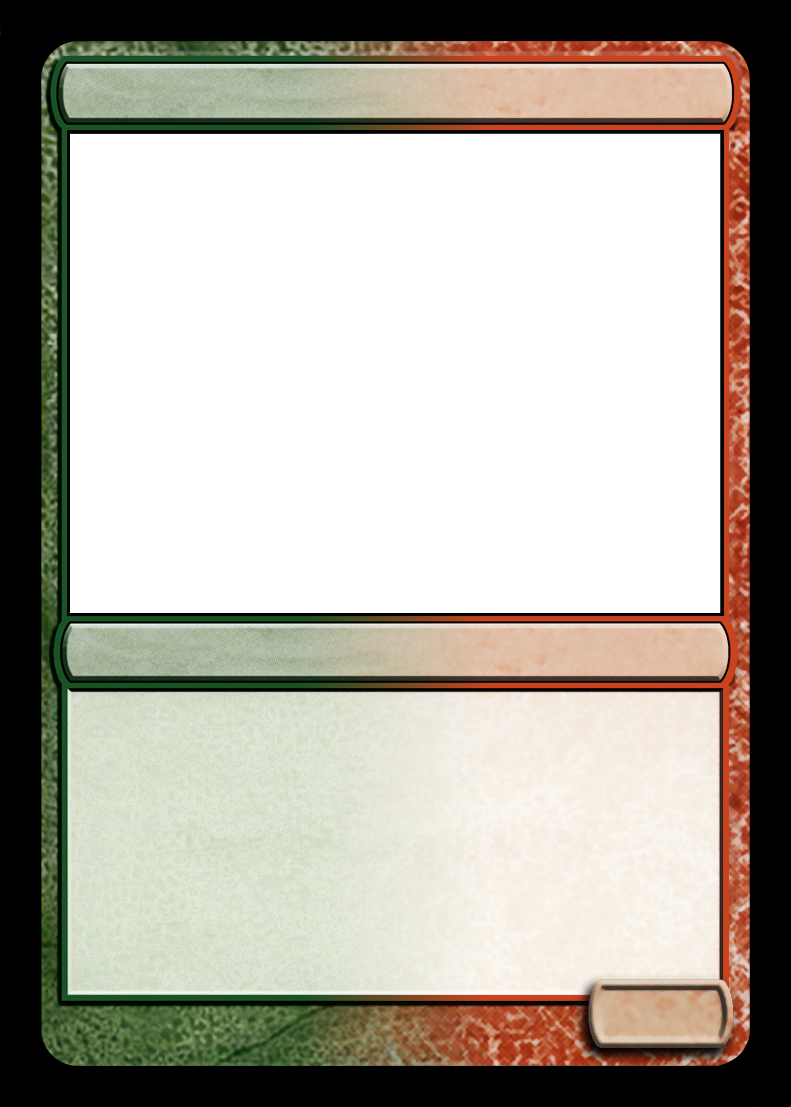
\includegraphics[width=\cardwidth cm, height=\cardheight cm]{fonds/fond_hybride.png}};

    %Titre
	\node[anchor=center] at (\titleX,\titleY) {\titlefont SRR};

	%Image
	\node[anchor=center] at (\imageX,\imageY) {
\includegraphics[width=\imageWidth px, height=\imageHeight px]{images/UO_18_VDD.jpg}};
	\node[anchor=center] at (6.1,4.5) {
\includegraphics[width=12 px, height=6 px]{fonds2/legacy.jpg}};

	%Type
	\node[anchor=center] at (\typeX,\typeY) {\typefont Bonus - Malus};

	%Description bonus
	\node[anchor=north west, text width=5.6cm] (description1) at (\descriptionX,\descriptionY) {\descriptionfont\setsize{7}(Bonus) Presque aucun trou dans la raquette. Avouez qu'un cryptologue vous a aidé hein ? L'ingénieur système défausse une carte.\par};

	%Description malus
	\node[anchor=north west, text width=5.6cm, below = 1pt of description1] (description2) {\descriptionfont\setsize{7}(Malus) Jouez cette carte contre l'Ingénieur Système. Pas de versionnage, rien n'est cohérent. Vous vous foutez du monde, cela mérite bien de piocher une carte !\par};

	%Separateur !!!!!PAS TOUCHE!!!!!
	\fill[black,path fading=west] (description1.south west) rectangle (description2.north);
	\fill[black,path fading=east] (description2.north) rectangle (description1.south east);

	%Numéro !!!!!PAS TOUCHE!!!!!
	\node[anchor=center] at (\numberX,\numberY) {\numberfont \cardnumber};
\end{tikzpicture}\verso %Verso


\begin{tikzpicture} %Recto
	%Fond
    \node[anchor=south west,inner sep=0] (carte) at (0,0) {
\includegraphics[width=7.1 cm, height=9.6 cm]{fonds/noir.png}};
    \node[anchor=center] at (carte.center) {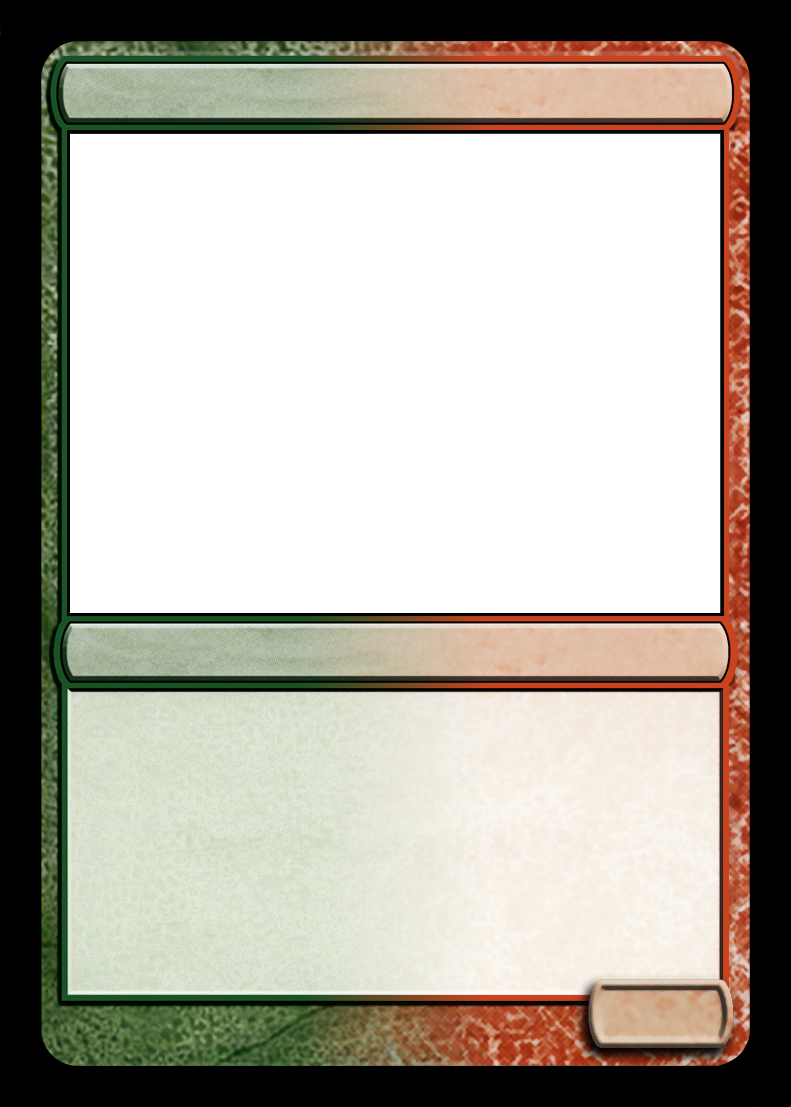
\includegraphics[width=\cardwidth cm, height=\cardheight cm]{fonds/fond_hybride.png}};

    %Titre
	\node[anchor=center] at (\titleX,\titleY) {\titlefont My beloved HoD};

	%Image
	\node[anchor=center] at (\imageX,\imageY) {
\includegraphics[width=\imageWidth px, height=\imageHeight px]{images/hod.jpg}};
	\node[anchor=center] at (6.1,4.5) {
\includegraphics[width=12 px, height=6 px]{fonds2/legacy.jpg}};

	%Type
	\node[anchor=center] at (\typeX,\typeY) {\typefont Bonus - Malus};

	%Description bonus
	\node[anchor=north west, text width=5.6cm] (description1) at (\descriptionX,\descriptionY) {\descriptionfont\setsize{6}(Bonus) Votre équipe est dynamique, reconnue du client et de votre hiérarchie. Tout cela grâce à votre management éclairé, ou alors ils sont très autonomes, ce qui indique un sens aigû du recrutement. Même si votre génie vous fatigue, le manager défausse une carte.\par};

	%Description malus
	\node[anchor=north west, text width=5.6cm, below = 1pt of description1] (description2) {\descriptionfont\setsize{6}(Malus) Plan de charge inconsistant, EAA en retard à base de sauvages copiés/collés. Le manager pioche une carte.\par};
	%Punchline
	\node[anchor=north west, text width=5.6cm, below = 33pt of description] (punchline) {\punchlinefont\setsize{6}``- My name is Doe, Garry Doe.''\par};
	
	%Separateur !!!!!PAS TOUCHE!!!!!
	\fill[black,path fading=west] (description1.south west) rectangle (description2.north);
	\fill[black,path fading=east] (description2.north) rectangle (description1.south east);

	%Numéro !!!!!PAS TOUCHE!!!!!
	\node[anchor=center] at (\numberX,\numberY) {\numberfont \cardnumber};
\end{tikzpicture}\verso %Verso


\begin{tikzpicture} %Recto
	%Fond
    \node[anchor=south west,inner sep=0] (carte) at (0,0) {
\includegraphics[width=7.1 cm, height=9.6 cm]{fonds/noir.png}};
    \node[anchor=center] at (carte.center) {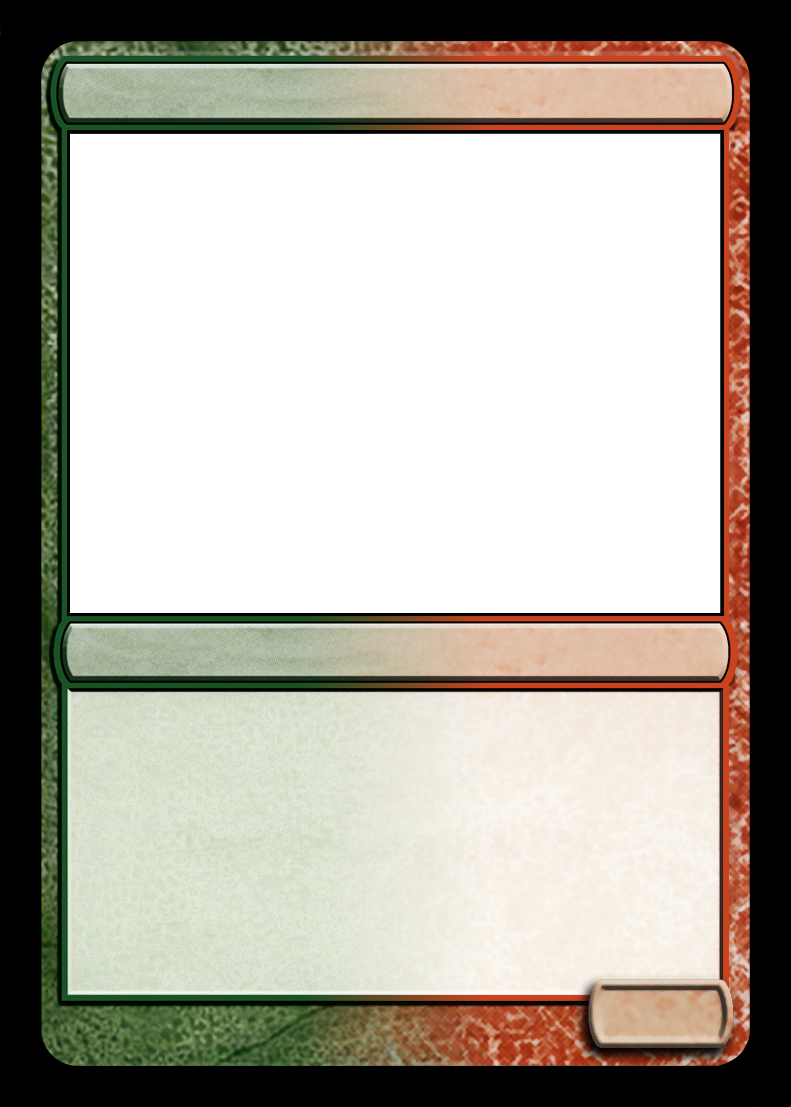
\includegraphics[width=\cardwidth cm, height=\cardheight cm]{fonds/fond_hybride.png}};

    %Titre
	\node[anchor=center] at (\titleX,\titleY) {\titlefont STR (Software Test Review)};

	%Image
	\node[anchor=center] at (\imageX,\imageY) {
\includegraphics[width=\imageWidth px, height=\imageHeight px]{images/developpement_code.jpg}};
	\node[anchor=center] at (6.1,4.5) {
\includegraphics[width=12 px, height=6 px]{fonds2/legacy.jpg}};

	%Type
	\node[anchor=center] at (\typeX,\typeY) {\typefont Bonus - Malus};

	%Description bonus
	\node[anchor=north west, text width=5.6cm] (description1) at (\descriptionX,\descriptionY) {\descriptionfont\setsize{7}(Bonus) Vous êtes tellement bon qu'on devrait carrément skipper la phase d'IVQ. Le développeur pioche une carte.\par};
	%Description malus
	\node[anchor=north west, text width=5.6cm, below = 1pt of description1] (description2) {\descriptionfont\setsize{7}(Malus) Ca ne compile pas, c'est truffé de bug, vous travailliez sur autre chose en douce n'est-ce pas ? Piochez une carte pour la peine.\par};
	%Punchline
	\node[anchor=north west, text width=5.6cm, below = 29pt of description] (punchline) {\punchlinefont\setsize{7}``{  gcc *.c -o \$EXE -Wall -brainfuck}''\par};
	%Separateur !!!!!PAS TOUCHE!!!!!
	\fill[black,path fading=west] (description1.south west) rectangle (description2.north);
	\fill[black,path fading=east] (description2.north) rectangle (description1.south east);

	%Numéro !!!!!PAS TOUCHE!!!!!
	\node[anchor=center] at (\numberX,\numberY) {\numberfont \cardnumber};
\end{tikzpicture}\verso %Verso


\begin{tikzpicture} %Recto
	%Fond
    \node[anchor=south west,inner sep=0] (carte) at (0,0) {
\includegraphics[width=7.1 cm, height=9.6 cm]{fonds/noir.png}};
    \node[anchor=center] at (carte.center) {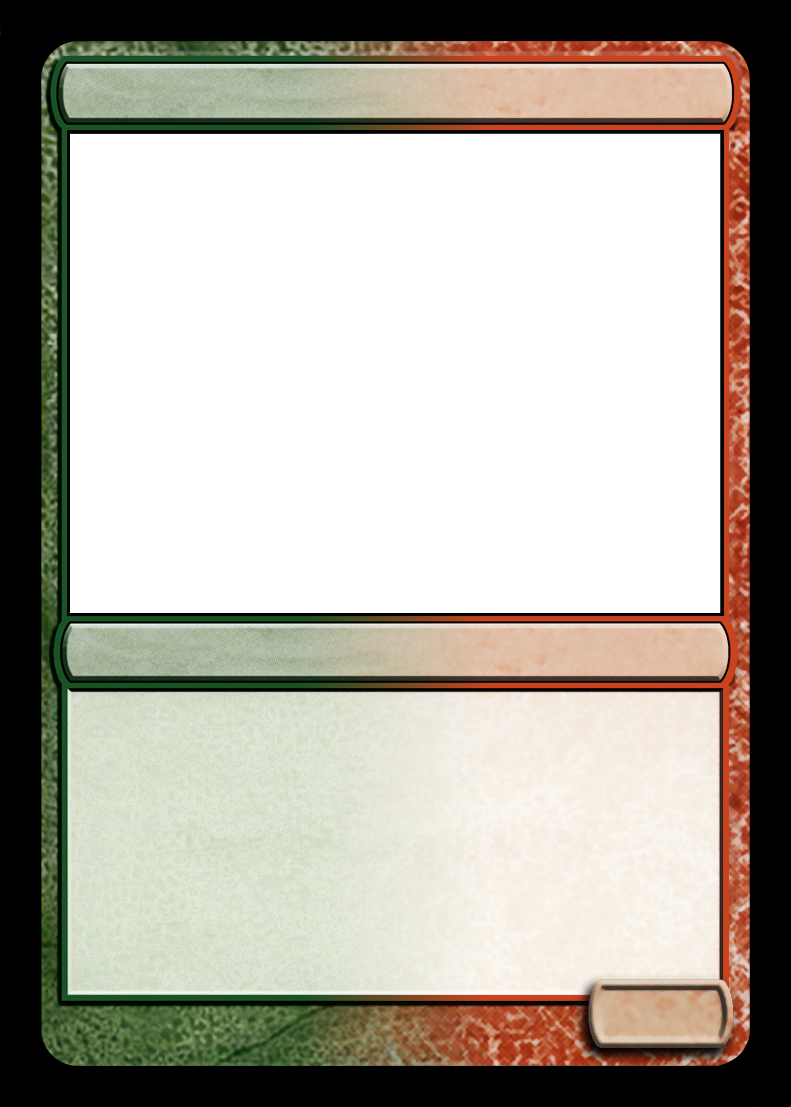
\includegraphics[width=\cardwidth cm, height=\cardheight cm]{fonds/fond_hybride.png}};

    %Titre
	\node[anchor=center] at (\titleX,\titleY) {\titlefont Jeudi de la sécurité};

	%Image
	\node[anchor=center] at (\imageX,\imageY) {
\includegraphics[width=\imageWidth px, height=\imageHeight px]{images/UO_22_marketing.jpg}};
	\node[anchor=center] at (6.1,4.5) {
\includegraphics[width=12 px, height=6 px]{fonds2/legacy.jpg}};

	%Type
	\node[anchor=center] at (\typeX,\typeY) {\typefont Bonus - Malus};

	%Description bonus
	\node[anchor=north west, text width=5.6cm] (description1) at (\descriptionX,\descriptionY) {\descriptionfont\setsize{6}(Bonus) Le marketting défausse une carte pour une présentation presque sans approximations d'une thématique technique à laquelle il ne maîtrise rien.\par};
	%Description malus
	\node[anchor=north west, text width=5.6cm, below = 1pt of description1] (description2) {\descriptionfont\setsize{6}(Malus) Vous n'avez pas réalisé que vous êtes en train de faire la promotion d'une librairie de la concurrence. Cela mérite bien de piocher une carte et lire quelques articles Wikipedia.\par};
	%Punchline
	\node[anchor=north west, text width=5.6cm, below = 29pt of description] (punchline) {\punchlinefont\setsize{6}``Pour cette punchline, voir avec le marketting.''\par};
	%Separateur !!!!!PAS TOUCHE!!!!!
	\fill[black,path fading=west] (description1.south west) rectangle (description2.north);
	\fill[black,path fading=east] (description2.north) rectangle (description1.south east);

	%Numéro !!!!!PAS TOUCHE!!!!!
	\node[anchor=center] at (\numberX,\numberY) {\numberfont \cardnumber};
\end{tikzpicture}\verso %Verso

\begin{tikzpicture} %Recto
	%Fond
    \node[anchor=south west,inner sep=0] (carte) at (0,0) {
\includegraphics[width=7.1 cm, height=9.6 cm]{fonds/noir.png}};
    \node[anchor=center] at (carte.center) {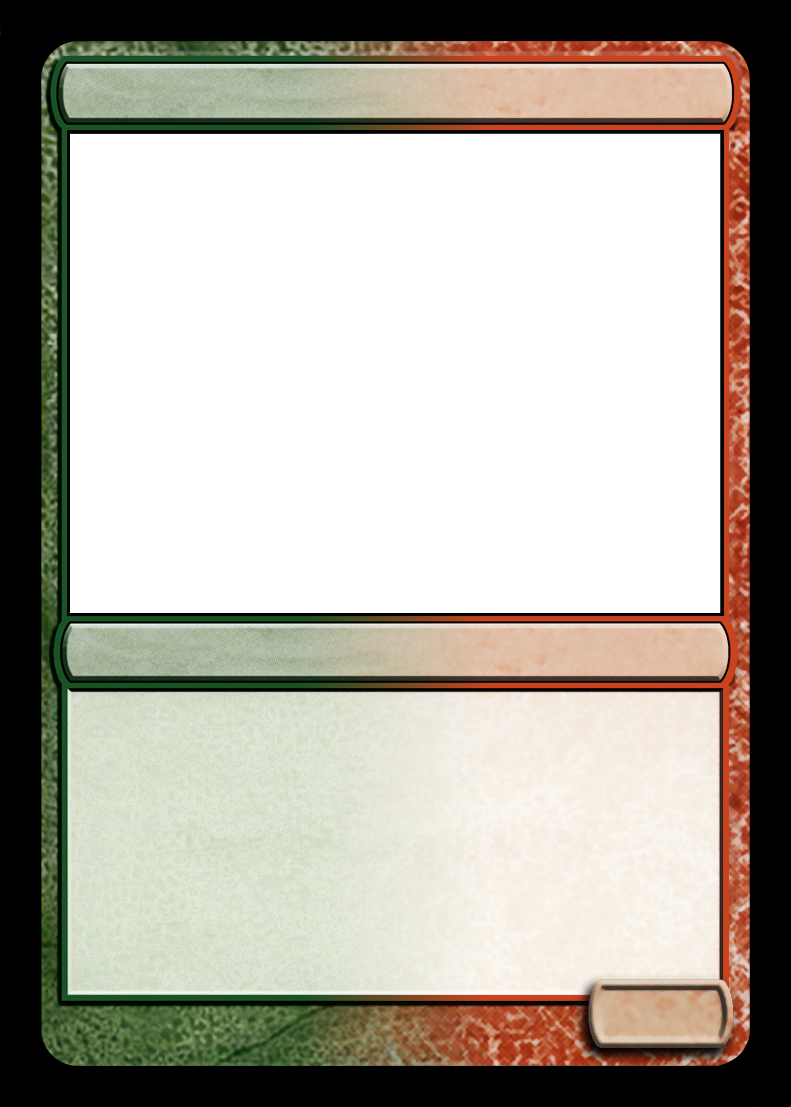
\includegraphics[width=\cardwidth cm, height=\cardheight cm]{fonds/fond_hybride.png}};

    %Titre
	\node[anchor=center] at (\titleX,\titleY) {\titlefont Proposition de thèse};

	%Image
	\node[anchor=center] at (\imageX,\imageY) {
\includegraphics[width=\imageWidth px, height=\imageHeight px]{images/UO_23_stage.jpg}};
	\node[anchor=center] at (6.1,4.5) {
\includegraphics[width=12 px, height=6 px]{fonds2/legacy.jpg}};

	%Type
	\node[anchor=center] at (\typeX,\typeY) {\typefont Bonus - Malus};

	%Description bonus
	\node[anchor=north west, text width=5.6cm] (description1) at (\descriptionX,\descriptionY) {\descriptionfont\setsize{7}(Bonus) Le stagiaire obtient automatiquement un CDI à ce tour (nouveau contrat).\par};
	%Description malus
	\node[anchor=north west, text width=5.6cm, below = 1pt of description1] (description2) {\descriptionfont\setsize{7}(Malus) Un CDI extérieur est proposé à ce petit ingrat de stagiaire qui accepte le poste ! Il ne peut y avoir de nouveau contrat à ce tour.\par};
	%Punchline
	\node[anchor=north west, text width=5.6cm, below = 27pt of description] (punchline) {\punchlinefont\setsize{7}``Je suis de la génération Y, je mérite bien plus que cette grille d'embauche.''\par};

	%Separateur !!!!!PAS TOUCHE!!!!!
	\fill[black,path fading=west] (description1.south west) rectangle (description2.north);
	\fill[black,path fading=east] (description2.north) rectangle (description1.south east);

	%Numéro !!!!!PAS TOUCHE!!!!!
	\node[anchor=center] at (\numberX,\numberY) {\numberfont \cardnumber};
\end{tikzpicture}\verso %Verso


\begin{tikzpicture} %Recto
	%Fond
    \node[anchor=south west,inner sep=0] (carte) at (0,0) {
\includegraphics[width=7.1 cm, height=9.6 cm]{fonds/noir.png}};
    \node[anchor=center] at (carte.center) {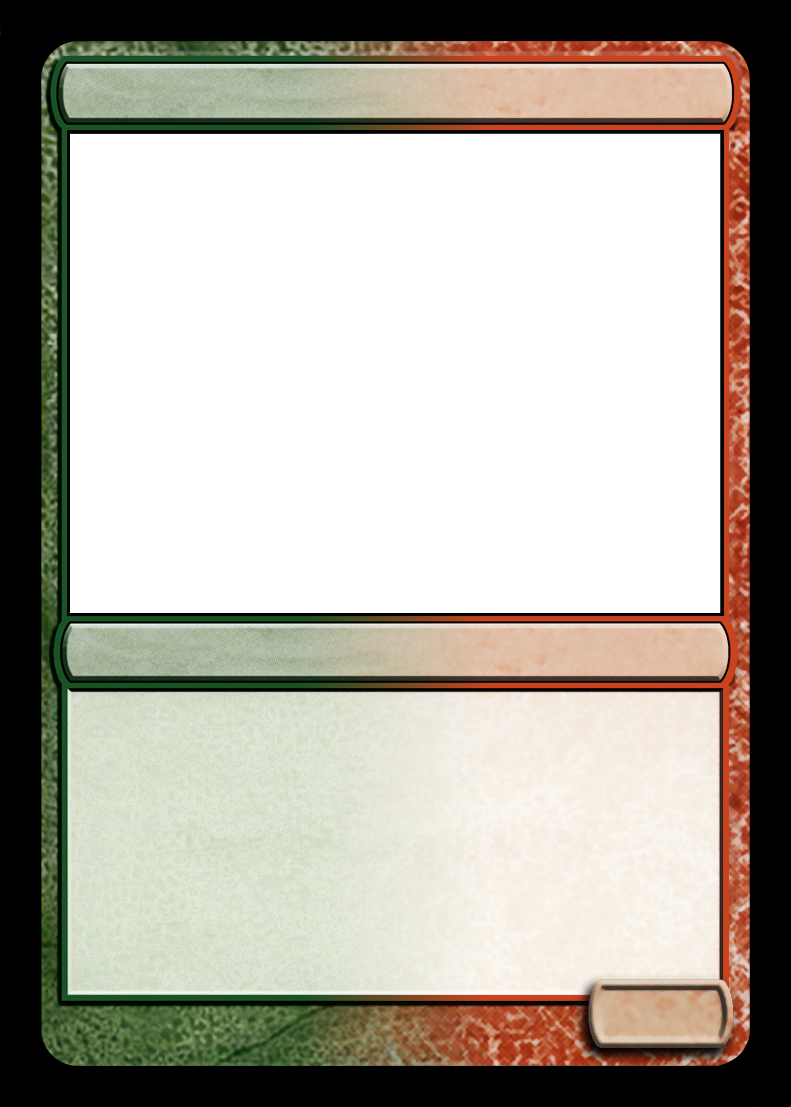
\includegraphics[width=\cardwidth cm, height=\cardheight cm]{fonds/fond_hybride.png}};

    %Titre
	\node[anchor=center] at (\titleX,\titleY) {\titlefont Demande KiSS refusée !};

	%Image
	\node[anchor=center] at (\imageX,\imageY) {
\includegraphics[width=\imageWidth px, height=\imageHeight px]{images/UO_24_kiss.jpg}};
	\node[anchor=center] at (6.1,4.5) {
\includegraphics[width=12 px, height=6 px]{fonds2/legacy.jpg}};

	%Type
	\node[anchor=center] at (\typeX,\typeY) {\typefont Bonus - Malus};

	%Description bonus
	\node[anchor=north west, text width=5.6cm] (description1) at (\descriptionX,\descriptionY) {\descriptionfont\setsize{6}(Bonus) Gnark gnark gnark. Cela a beau être votre quotidien de DSI, ça vous fait toujours autant plaisir. Seul DSI peut jouer cette carte pour forcer un autre joueur à piocher.\par};
	%Description malus
	\node[anchor=north west, text width=5.6cm, below = 1pt of description1] (description2) {\descriptionfont\setsize{6}(Malus) Mais, mais, mais, non ! Cet utilisateur obstiné réémet sa demande pour la dixième fois. Ce surcroît de travail épuise le joueur DSI qui pioche une carte.\par};
	%Punchline
	\node[anchor=north west, text width=5.6cm, below = 27pt of description] (punchline) {\punchlinefont\setsize{6}``N'oubliez pas de remplir notre questionnaire de satisfaction.''\par};

	%Separateur !!!!!PAS TOUCHE!!!!!
	\fill[black,path fading=west] (description1.south west) rectangle (description2.north);
	\fill[black,path fading=east] (description2.north) rectangle (description1.south east);

	%Numéro !!!!!PAS TOUCHE!!!!!
	\node[anchor=center] at (\numberX,\numberY) {\numberfont \cardnumber};
\end{tikzpicture}\verso %Verso
%%%%%%%%%%%%%%%%%%%%%%%%%%%%%%%%%%%%%%%%%%%%%

\begin{tikzpicture} %Recto
	%Fond
    \node[anchor=south west,inner sep=0] (carte) at (0,0) {
\includegraphics[width=7.1 cm, height=9.6 cm]{fonds/noir.png}};
    \node[anchor=center] at (carte.center) {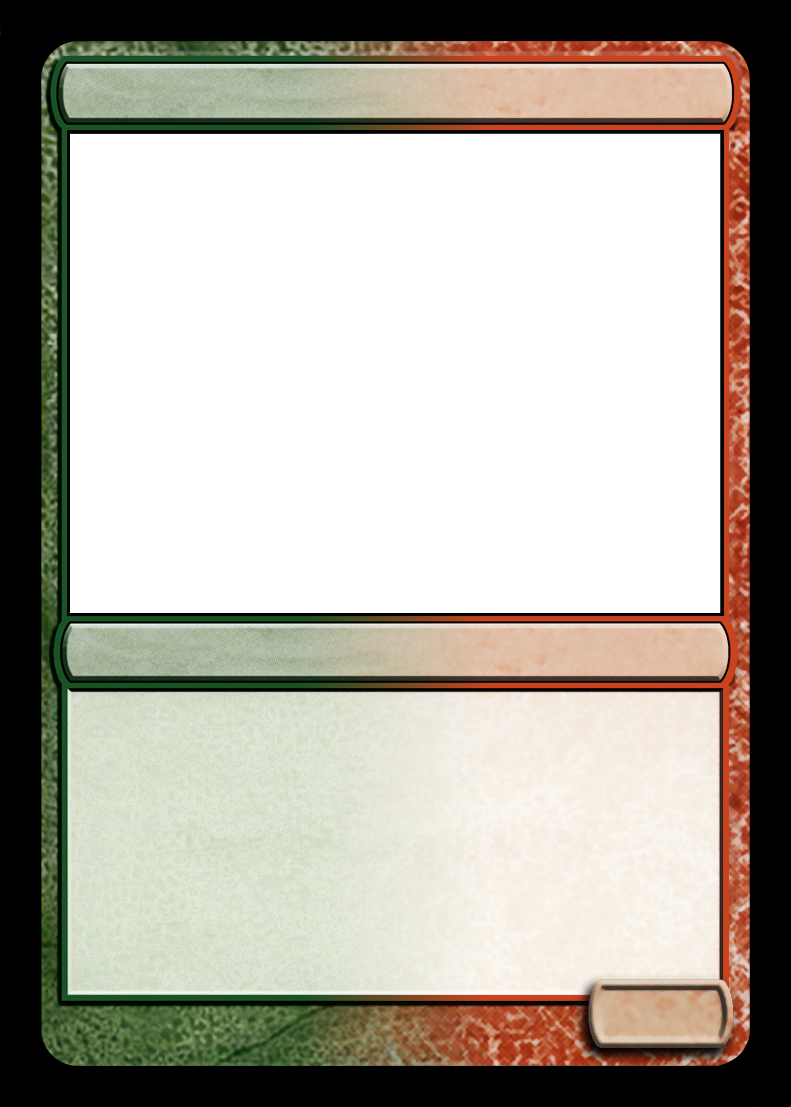
\includegraphics[width=\cardwidth cm, height=\cardheight cm]{fonds/fond_hybride.png}};

    %Titre
	\node[anchor=center] at (\titleX,\titleY) {\titlefont Invention géniale};

	%Image
	\node[anchor=center] at (\imageX,\imageY) {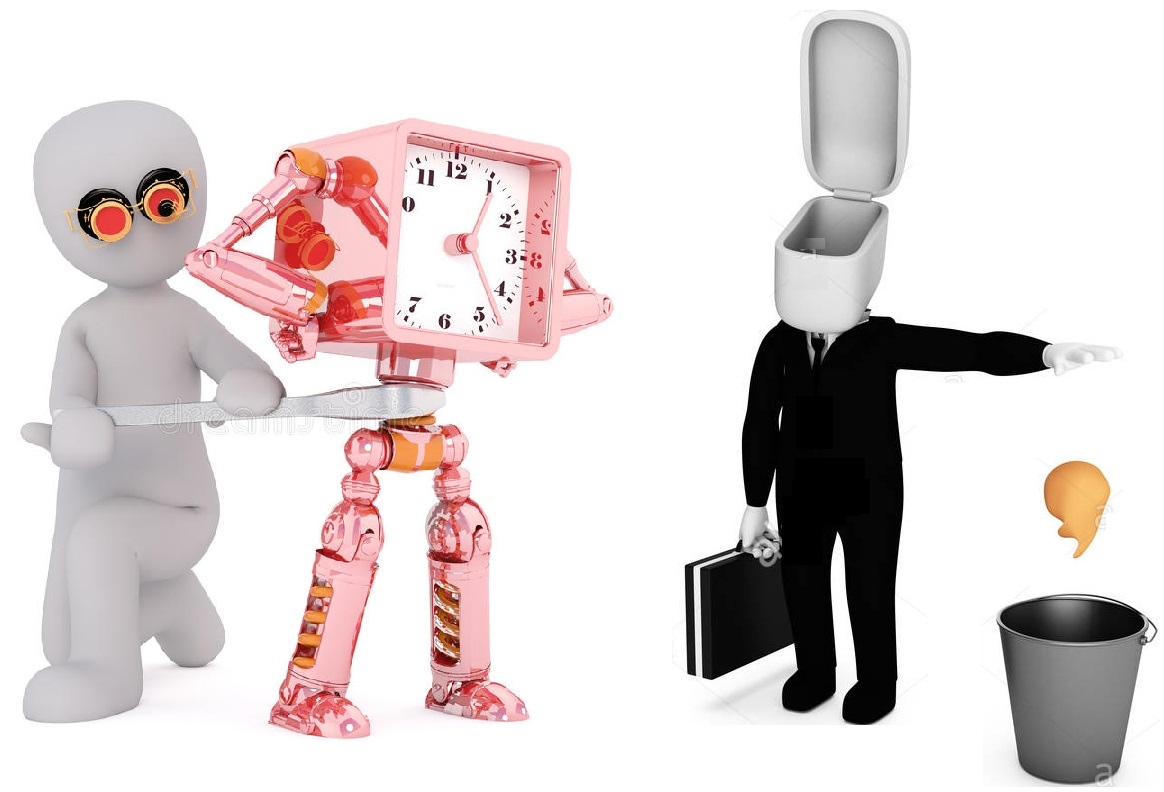
\includegraphics[width=\imageWidth px, height=\imageHeight px]{images/invention.jpg}};
	\node[anchor=center] at (6.1,4.5) {
\includegraphics[width=12 px, height=6 px]{fonds2/legacy.jpg}};

	%Type
	\node[anchor=center] at (\typeX,\typeY) {\typefont Bonus - Malus};

	%Description bonus
	\node[anchor=north west, text width=5.6cm] (description1) at (\descriptionX,\descriptionY) {\descriptionfont\setsize{7}(Bonus) Votre invention est clairement une opportunité majeure pour le groupe. Le cryptologue défausse une carte.\par};
	%Description malus
	\node[anchor=north west, text width=5.6cm, below = 1pt of description1] (description2) {\descriptionfont\setsize{7}(Malus) Bien sûr que c'est génial. Mais la priorité est de produire cette perforatrice de bande. Le cryptologue pioche une carte de désespoir.\par};
	%Punchline
	\node[anchor=north west, text width=5.6cm, below = 29pt of description] (punchline) {\punchlinefont\setsize{6}``THALES, innover aujourd'hui avec les technologies d'avant hier.''\par};

	%Separateur !!!!!PAS TOUCHE!!!!!
	\fill[black,path fading=west] (description1.south west) rectangle (description2.north);
	\fill[black,path fading=east] (description2.north) rectangle (description1.south east);

	%Numéro !!!!!PAS TOUCHE!!!!!
	\node[anchor=center] at (\numberX,\numberY) {\numberfont \cardnumber};
\end{tikzpicture}\verso %Verso999

%%%%%%%%%%%%%%%%%%%%%%%%%%%%%%%%%%%%%%%%%%%%%
\begin{tikzpicture} %Recto
	%Fond
    \node[anchor=south west,inner sep=0] (carte) at (0,0) {
\includegraphics[width=7.1 cm, height=9.6 cm]{fonds/noir.png}};
    \node[anchor=center] at (carte.center) {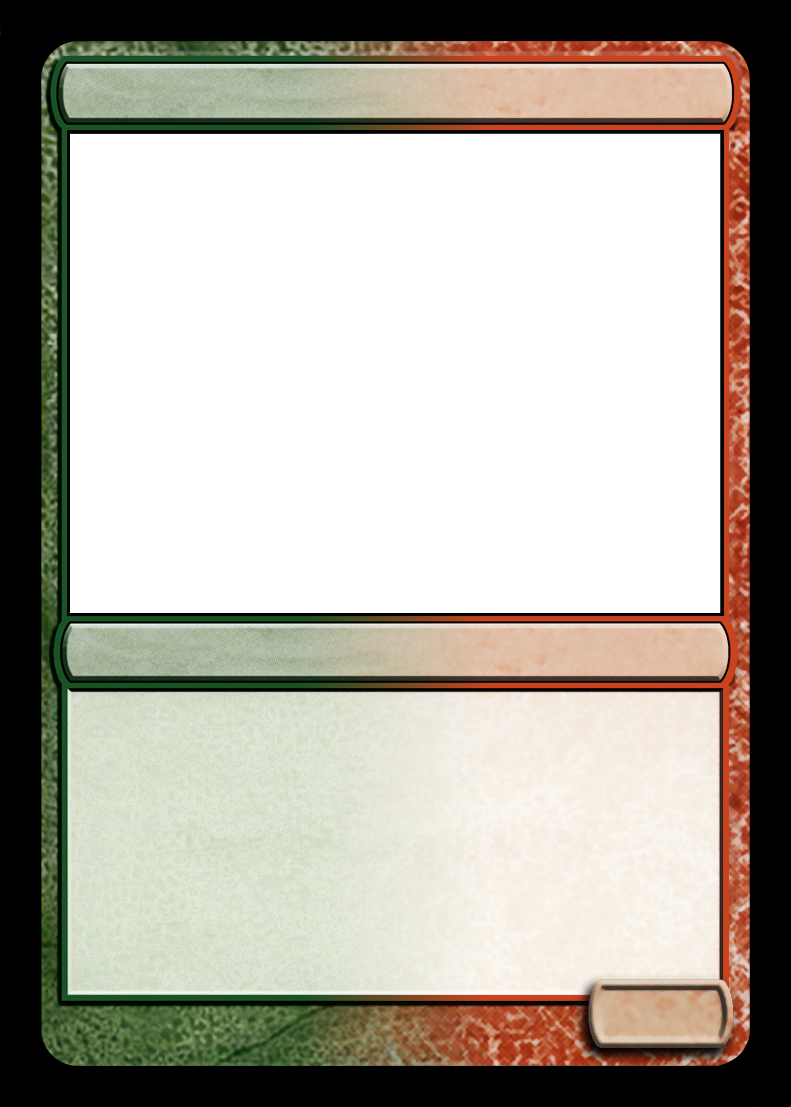
\includegraphics[width=\cardwidth cm, height=\cardheight cm]{fonds/fond_hybride.png}};

    %Titre
	\node[anchor=center] at (\titleX,\titleY) {\titlefont Journée des imputations};

	%Image
	\node[anchor=center] at (\imageX,\imageY) {
\includegraphics[width=\imageWidth px, height=\imageHeight px]{images/Jourput.jpg}};
	\node[anchor=center] at (6.1,4.5) {
\includegraphics[width=12 px, height=6 px]{fonds2/legacy.jpg}};

	%Type
	\node[anchor=center] at (\typeX,\typeY) {\typefont Bonus - Malus};

	%Description bonus
	\node[anchor=north west, text width=5.6cm] (description1) at (\descriptionX,\descriptionY) {\descriptionfont\setsize{8}(Bonus) Tous ces numéros donnent un sens à l'existence du PMO qui défausse une carte.\par};
	%Description malus
	\node[anchor=north west, text width=5.6cm, below = 1pt of description1] (description2) {\descriptionfont\setsize{8}(Malus) L'OS est fermé, c'est affecté sur le mauvais projet. Quel bazar pour le PMO qui pioche une carte.\par};
	%Punchline
	\node[anchor=north west, text width=5.6cm, below = 25pt of description] (punchline) {\punchlinefont\setsize{6}``A remplir à la fin du mois. Donc le 15.''\par};

	%Separateur !!!!!PAS TOUCHE!!!!!
	\fill[black,path fading=west] (description1.south west) rectangle (description2.north);
	\fill[black,path fading=east] (description2.north) rectangle (description1.south east);

	%Numéro !!!!!PAS TOUCHE!!!!!
	\node[anchor=center] at (\numberX,\numberY) {\numberfont \cardnumber};
\end{tikzpicture}\verso %Verso999